\documentclass[amsmath,amssymb,aps,twocolumn,nofootinbib]{revtex4-2}

\usepackage{bm}
\usepackage{graphicx}
\usepackage[colorlinks=true]{hyperref}

\newcommand{\braket}[1]{\left \langle #1 \right \rangle}
\newcommand{\parens}[1]{\left ( #1 \right )}
\newcommand{\jtd}[1]{{\color{red}\textbf{JTD: #1}}}

\begin{document}
\title{Magnetic Phase Transitions in an Aperiodic Monotile}
\author{Jack Dinsmore}
\affiliation{Department of Physics, Stanford University}

\begin{abstract}
  A family of shapes known as ``einstein tiles'' has been discovered which tile the plane aperiodically. We define the Ising, XY, and Heisenberg models on the einstein tilings and compute the magnetization and susceptibility of the tiling as a function of temperature using Monte Carlo methods. This allows us to produce phase diagrams of the relationship between the critical temperature of the tiling and the dimensions of the einstein tile.
\end{abstract}

\maketitle

\section{Introduction}
The Ising model was one of the first statistical mechanics models to contain a phase transition, and remains one of the only exactly solvable examples. It consists of defining a variable $s_i = \pm 1$ at every site of a lattice with $N$ sites as a classical approximation of the up-or-down spin of a fermion. On further analogy with fermionic spins, it asserts that the spins interact by defining the classical Hamiltonian
\begin{equation}
  H = -J \sum_{\braket{ij}} s_i s_j + h \sum_i s_i
  \label{eqn:ising}
\end{equation}
where $h$ is an applied magnetic field. This model's phase transition is most visible in the magnetization, defined as
\begin{equation}
  M = \frac{1}{N}\braket{\sum_{i} s_i}
  \label{eqn:magnetization}
\end{equation}
where the brackets indicate an average over the statistical ensemble of states, weighted by the Boltzmann factor $e^{-\beta H}$.

The phase transition occurs for the following reason. For $h=0$, the Hamiltonian displays $s_i\rightarrow -s_i$ symmetry. If the thermodynamic system explores all of phase space, then the average thermodynamic state should possess the same symmetries of the Hamiltonian so that $M=0$. However, for low temperature we also expect the system to attain the lowest possible energy. This state consists of all spins up (or all spins down) has $M = 1$ (or $-1$), which violates the expectation of no magnetization. The resolution to this apparent contradiction that there exists a critical temperature $T_c$ below which energetic considerations dominate and the crystal is magnetic ($|M|>0$), and above which the symmetry of phase space dominates and the crystal is not magnetic ($M = 0$).

The phenomenon of critical temperature has been generalized to other theories. In particular, if the system's variables are arranged as a members of a field $s(\bm x)$, then the free energy may be approximated as an integral over functions of $s(\bm x)$. This approximation is called Landau Field Theory and it yields a form which is readily able to create phase transitions. Taking the Ising model as an example, we could approximate the $s_i$ spins defined on discrete points $x_i$ as the field $s(\bm x)$ defined for any position $\bm x$. The original Hamiltonian contained translational, rotational, and $s\rightarrow-s$ symmetry, and therefore the free energy should as well. Expanding it in powers of $s(\bm x)$ guarantees the form
\begin{equation}
F \propto -\int d^d x \, \parens{(\nabla s(\bm x))^2 + A s(\bm x)^2 + B s(\bm x)^4 + \dots}
\label{eqn:landau}
\end{equation}
where $d$ is the number of dimensions of the lattice and $A$ and $B$ are arbitrary constants. If $A>0$, then free energy is minimized at every point by setting $s(\bm x)$. However, if $A<0$, then minimizing the free energy necessitates setting $s(\bm x)$ to some nonzero value, thereby magnetizing the crystal and creating a phase transition. In principle, all the parameters of the model including $A$ may depend on temperature. All that is necessary to describe a phase transition is therefore to write a form of $A$ which allows it to cross from positive to negative at a critical temperature $T_c$.

The utility of this field theory approximation is in its generality. All Ising-like models like it are Landau field theories and are all described by Eq~\ref{eqn:landau}, meaning they have the same near-critical-point behavior. This statement is independent of the lattice or interaction strengths; it depends only on the field $\bm s$ and the dimensionality of the lattice. A particular lattice's only unique properties its its values of $A$ and $B$; i.e., the value of its critical temperature.

The solution to a spin model depends on the lattice on which the model is defined. For example, an exact solution exists for the two-dimensional Ising model defined on the square lattice which yields an exact formula for the critical temperature. In the absence of a full solution, a series expansions in $\beta$ (valid at high temperature) or $e^{-\beta}$ (valid at low temperature) can be written for the model's thermodynamical quantities. For self-dual lattices such as the square lattice, the coefficients of the high- and low-temperature expansions are the same --- a phenomenon known as Kramers-Wannier duality \cite{kramers}. This duality leads to an analytical solution for the critical temperature even in the absence of a full solution. Even for lattices which are not self-dual, it is sometimes possible to use a similar technique to relate the series expansions of the lattice and its dual to each other. This can be done for the hexagonal lattice, for example, which is dual to the triangular lattice \cite{bhattacharjee1995fifty}.

In more complicated crystals, however, the only available approaches to computing $T_c$ are numerical. For example, the Penrose lattice consists of two tiles which fill the two-dimensional plane aperiodically, making it difficult to model the system analytically. Ref. \cite{penrose-ising} computes magnetism as a function of temperature using numerical methods and finds that the aperiodic nature of the lattice does not affect the physics at a qualitative level, since $M(T)$ inherits most of its properties from the very general Landau theory.

Recently, the first \textit{single} tile which fills the plane aperiodically has been discovered, and named the einstein tile (German for ``one stone'') (figure \ref{fig:einstein}) \cite{smith2023aperiodic}. An interesting fact about the einstein tile is that its dimensions are adjustable. The tile consists of two side lengths $a$ and $b$, and any ratio of $a/b$ leads to an aperiodic tiling except $a/b=0$, 1, or $\infty$. If we treat the spin-spin interaction as weaker across the longer bonds, then this $a/b$ ratio represents a free parameter of the crystal, so that the critical temperature is a function of $a/b$. The phase diagram of $T_c(a/b)$ is therefore an intrinsic property of the einstein tiling, more so than the commonplace behavior of $M(T)$.

\begin{figure}
  \centering
  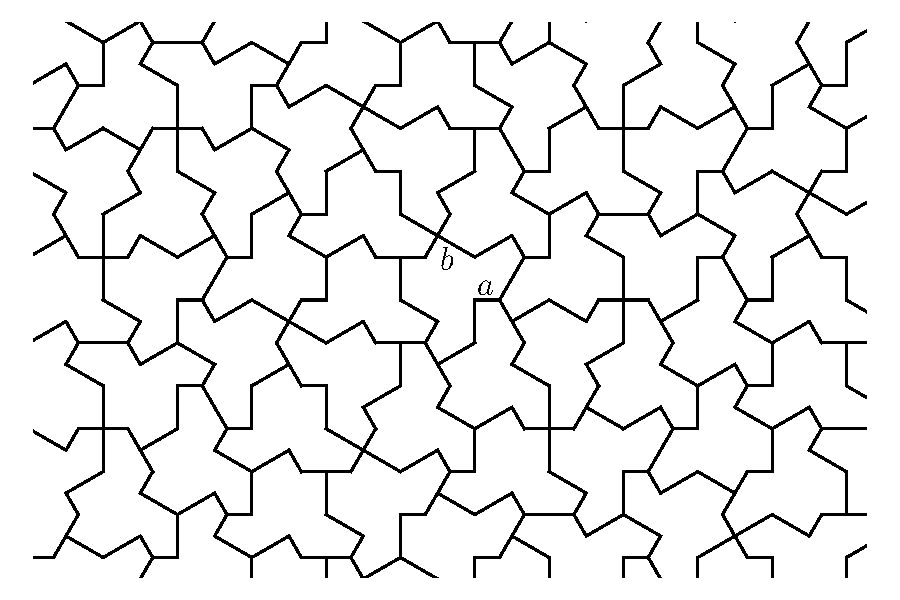
\includegraphics[width=\linewidth]{../figs/einstein.pdf}
  \caption{The einstein tiling}
  \label{fig:einstein}
\end{figure}

In this final project, we use numerical methods to compute the phase diagram $T_c(a/b)$ for the einstein tile under the Ising model and two similar models. We also compute the phase diagram for a rectangular lattice with bond lengths $a$ and $b$ to compare to the einstein lattice phase diagram, later using this calculation to solve for the one-dimensional transverse Ising model phase transition. The structure of the paper is as follows: in section \ref{sec:spin-models}, we briefly review the spin models. In section \ref{sec:wolff} we discuss the numerical methods used to compute $T_c$. We present the phase diagrams in section \ref{sec:results}, followed by section \ref{sec:tim} on the transverse Ising model. We conclude with section \ref{sec:conclusion}.


\section{Spin models}
\label{sec:spin-models}

In addition to the Ising model Hamiltonian (Eq.~\ref{eqn:ising}), we study the XY model which consists of promoting $s_i$ to a two-dimensional unit vector defined at every lattice point. The interaction term in the Hamiltonian becomes $\bm s_i \cdot \bm s_j$. This XY model has different $T_c$ than the Ising model and can even contain vortices, which are topologically protected quasi-particles where the curl of $\bm s_i$ is nonzero. A third spin model is the Heisenberg model, which is similar to the XY model except that $s_i$ is promoted to a three-dimensional unit vector. Unlike the XY model, the Heisenberg model may not display a true phase transition in the thermodynamic limit \cite{tomita2014finite}. Nevertheless, it has phase-transition-like behavior in that $M$ experiences a large drop in a small temperature range. The Ising, XY, and Heisenberg models have progressively more degrees of freedom, and their critical temperatures are therefore progressively lower.

A fourth spin model is the Transverse Ising Model (TIM), which consists of replacing $s_i$ in Eq.~\ref{eqn:ising} with the Pauli matrices $\bm \sigma_i$ and $\bm \sigma_j$ and interpreting the result as a quantum Hamiltonian. A simple proof using the path integral approach (appendix \ref{app:tim-equivalence}) shows that the $d$-dimensional TIM is equivalent to a classical Ising model in $d+1$ dimensions in the limit of a very strong interaction strength in the extra dimension. Thus, critical temperatures for all four of these models can be found using the same techniques.

Beyond the magnetization $M$, another interesting property of a spin model is its susceptibility $\chi = \frac{dM}{dh}$. Even in a model which sets $h=0$, $\chi$ an be defined as follows by the fluctuation-dissipation theorem (appendix \ref{app:fluctuation-dissipation}):
\begin{equation}
  \chi = \frac{\partial M}{\partial h} = \frac{1}{N}\braket{\sum_i(s_i - M)^2}.
\end{equation}
The susceptibility diverges at the critical temperature and otherwise falls off to zero.


\section{Cluster Monte Carlo Methods: the Wolff Algorithm}
\label{sec:wolff}

To find the critical temperature of the einstein lattice, we must numerically compute the ensemble average of Eq.~\ref{eqn:magnetization}. This average is extremely expensive to compute because the number of states in the ensemble is $2^N$ for the Ising model. However, approximate results can be obtained by computing the sum over a much smaller, random selection of states $K$. This approximation technique is called a Monte Carlo method.

The method of selecting states for $K$ is critical to the accuracy of a Monte Carlo method. It needs to add states $\psi$ to $K$ with some probability $P(\psi)$ which prefers states that are representative of the full ensemble, otherwise the convergence of the ensemble average will be poor. Many states are not representative, making it difficult to find a new state $\psi$ which has high enough $P(\psi)$ to be added to $K$. One way to resolve this problem is to make $\psi$ very similar to a state $\phi$ already in $K$. Assuming $\phi$ is representative of the ensemble, then $\psi$ is also likely to be represented by the ensemble. We then add $\psi$ to $K$ with some probability $P(\phi \rightarrow \psi)$, which is a function we discuss in the next paragraph. The technique of using previous states $\phi$ to create a new state $\psi$ is called a Markov Chain Monte Carlo method (MCMC).

For an MCMC to be correct, $P(\phi \rightarrow \psi)$ must be reversible, meaning that the probability to go from $\phi$ to $\psi$ must be equal to the probability to go from $\psi$ to $\phi$. This condition is necessary to prevent $K$ from getting stuck in an unrepresentative region of phase space. The probability to go from $\phi$ to $\psi$ is the probability for the MCMC to be at state $\phi$ in the first place times the probability to switch to $\psi$: $P(\phi \rightarrow \psi)P(\phi)$. Thus, detailed balance requires
\begin{equation}
  P(\phi \rightarrow \psi)P(\phi) = P(\psi \rightarrow \phi)P(\psi)
  \label{eqn:detailed-balance}
\end{equation}
Any method of generating a new state $\psi$ from the old state $\phi$ that satisfies Eq.~\ref{eqn:detailed-balance} is a valid MCMC.

There are many methods of generating new states, but the one we will use in this paper is the Wolff algorithm, which is known to converge well near the critical temperature \cite{wolff1989collective}. The algorithm generates a new state $\psi$ by probabilistically choosing a cluster of spins and then flipping all the spins at once. The cluster starts the cluster at a random location $i$. It then adds each neighbor $j$ to the cluster with probability
\begin{equation}
  P(i,j) = 1 - \exp\parens{\mathrm{min}\left[0, 2\beta s_i s_j \right]}.
  \label{eqn:wolff-algo}
\end{equation}
For every spin $j$ which was added to the cluster, it then uses the same equation to assign $j$'s neighbors to the cluster until every neighbor has been rejected. At that point, the cluster's spins are flipped to form the new state $\psi$. Ref.~\cite{wolff1989collective} confirms that Eq.~\ref{eqn:wolff-algo} satisfies the detailed balance constraint and therefore is a good MCMC.

For the XY model, Eq.~\ref{eqn:wolff-algo} must be modified to handle vector-valued spins. The approach is to choose a random vector $\bm r$ as a direction against which to compare to spins, so that
\begin{equation}
  P(i,j) = 1 - \exp\parens{\mathrm{min}\left[0, 2\beta J (\bm r \cdot \bm s_i)(\bm r \cdot \bm s_j) \right]}.
\end{equation}
For consistency, we keep $\bm r$ the same throughout the cluster, but for the next cluster we re-draw a new $\bm r$.

A third and final extension is necessary to the Wolff algorithm in order to handle quantum spin models. As mentioned above, the TIM in two dimensions is equivalent to the Ising model in three dimensions where interaction strengths $J$ are very strong in the new direction. We could therefore stack many two-dimensional crystals to form a three-dimensional crystal on which we run the Wolff algorithm, but this is inefficient because the large $J$ along the third axis will make the clusters grow large in this direction. Ref.~\cite{blote2002cluster} speeds up the process by analytically computing the behavior of the Wolff algorithm along the third axis in the limit of large $J$. The classical Wolff algorithm can then be run on the two-dimensional lattice while the spins on the third axis are set according to this analytical result.

\section{Phase Diagrams}
\label{sec:results}

We implemented the Wolff algorithm with a custom code base \footnote{\jtd{LINK}} and executed for a variety of spin models and crystals. Except when stated otherwise, we used a finite-size lattice with initial conditions of random spins. Magnetization $M$ and susceptibility $\chi$ measurements were collected every 16 cluster flips to prevent autocorrelation. 10,000 $M$ and $\chi$ measurements were made when $M$ was small, and when $M$ was large we made 1,000 measurements because the algorithm was found to be more stable for $T< T_c$.

The upper left panel of Figure \ref{fig:square} shows the magnetization $M$ and susceptibility $\chi$ of the Ising, XY, and Heisenberg models executed on a square lattice as a function of the lattice width $L = \sqrt{N}$. The magnetization drops rapidly near $T_c$, shown as vertical dotted lines. The location of these transitions is not perfect, and $M$ it is not strictly zero for $T<T_c$ due to finite-size effects. Larger lattice sizes lead to smaller $M$ for $T<T_c$. The XY and Heisenberg models have substantially lower $T_c$ due to the increased degrees of freedom of the spin system. Furthermore, $M$ approaches its low-temperature limit of 1 linearly for the Heisenberg and XY models, while the approach is exponential for the Ising model. This is a qualitative difference between the Ising and XY models.

\begin{figure*}
  \centering
  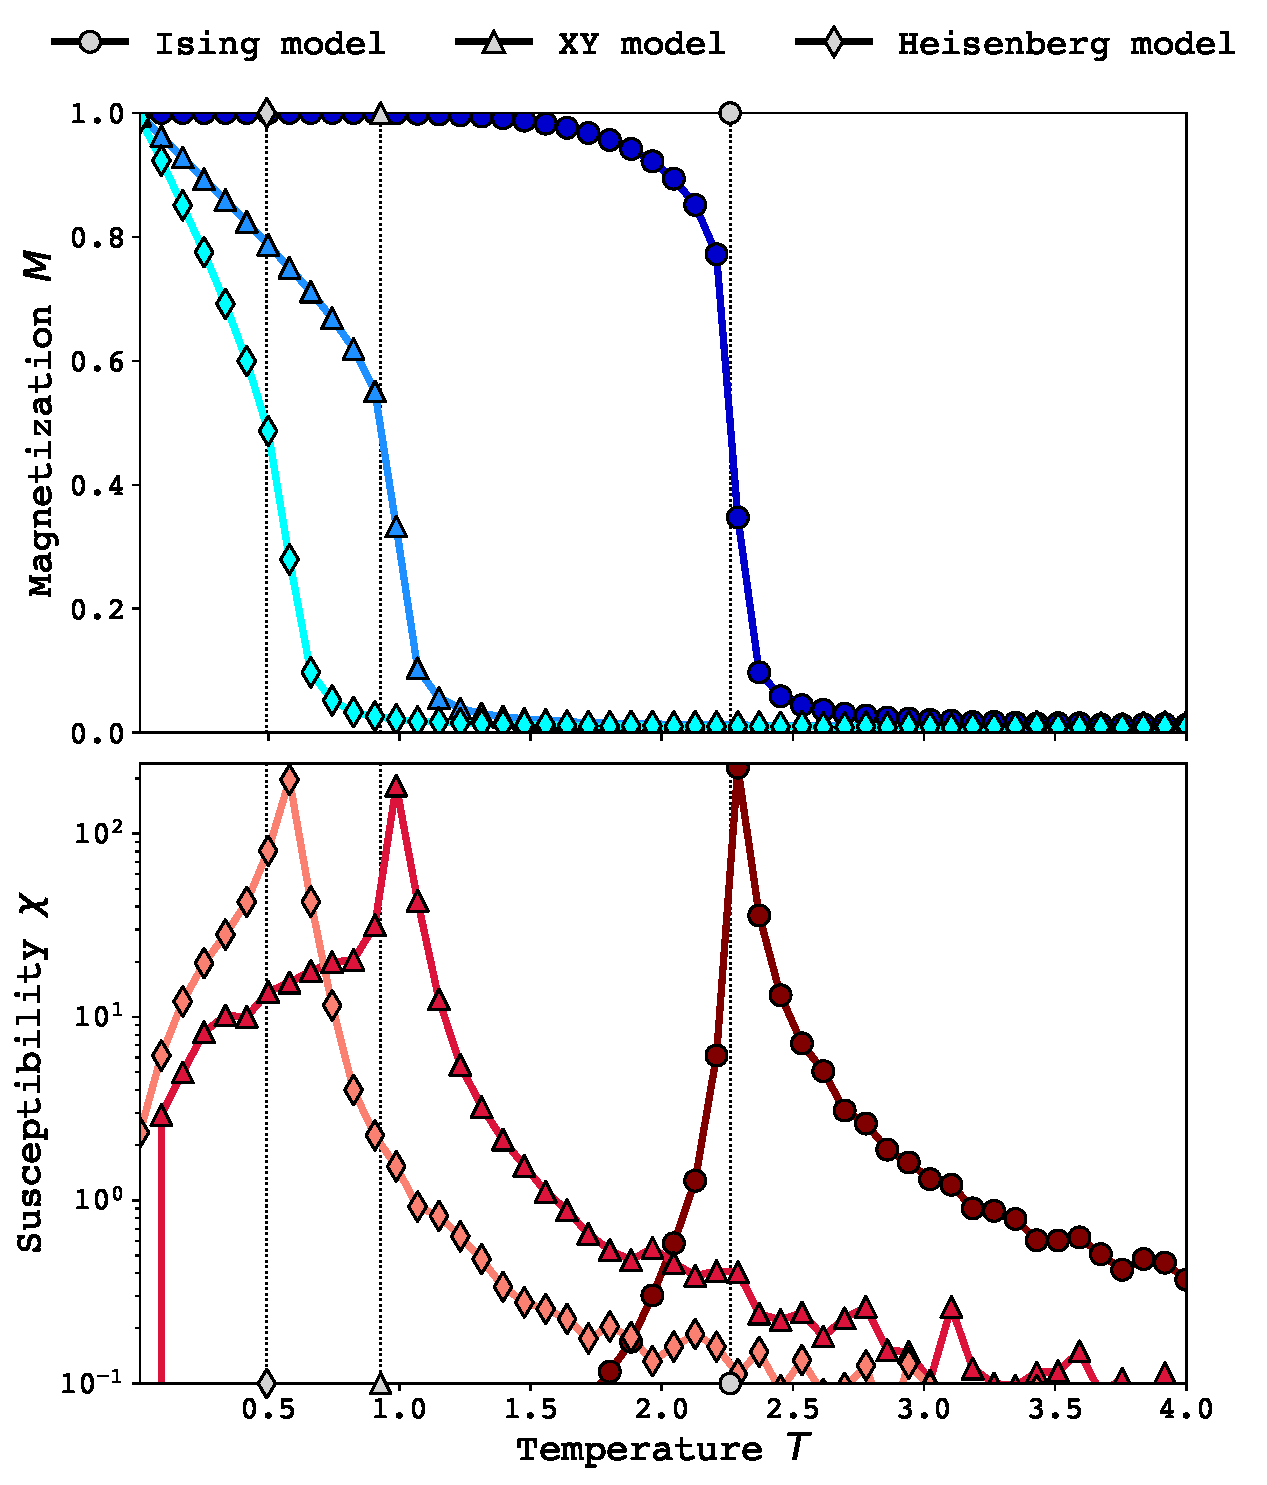
\includegraphics[width=0.49\linewidth]{../figs/square.pdf}\hfill
  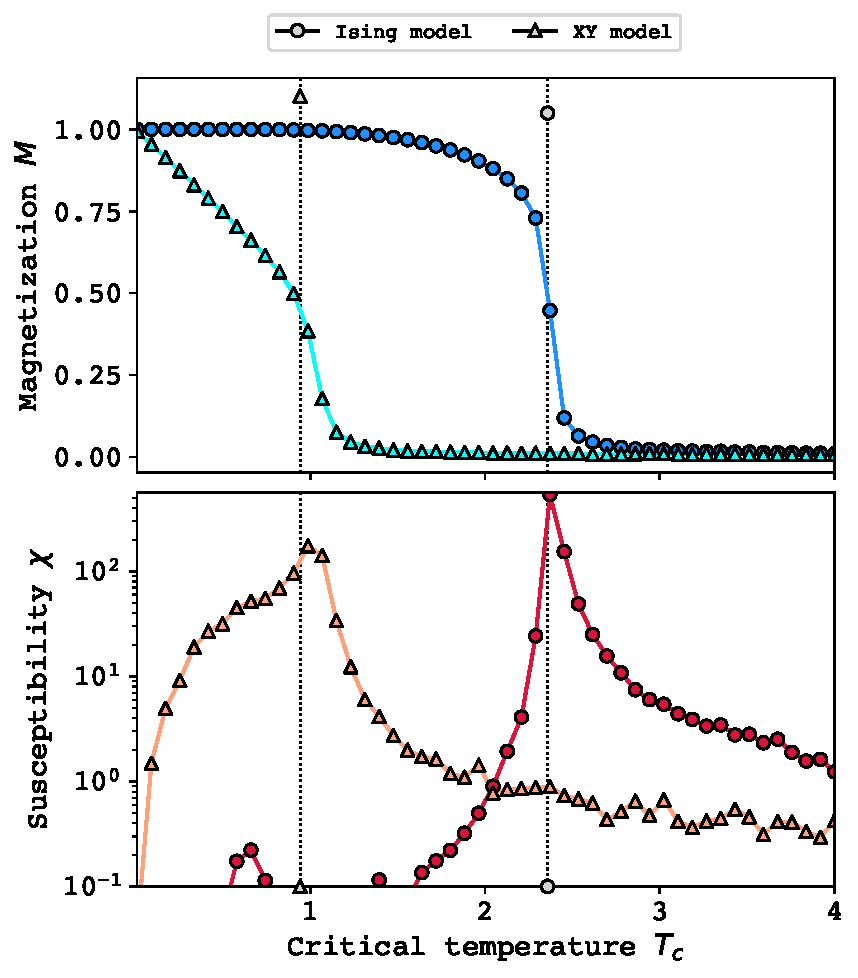
\includegraphics[width=0.49\linewidth]{../figs/penrose.pdf}
  \caption{Magnetization and susceptibility as a function of $T_c$ under the XY and Ising models. \textit{Left}: A square lattice with $N=128^2=16,384$ sites. \textit{Right}: A Penrose lattice with $N=21,316$ sites.}
  \label{fig:square}
\end{figure*}

The susceptibility in the bottom left panel produces a maximum at $T_c$, decaying to zero more rapidly on the low-temperature side than high-temperature. For an infinite lattice, the peak will be likewise infinite, but it is blunted by finite $N$. The peak in susceptibility can be used as a measure of the location of $T_c$, as can the point of maximum slope of $M$.

In both crystals and both models, the point of maximum susceptibility and maximum $dM/dT$ occur at approximately the same location. For the sake of approximating the critical temperature, we take the $T$ point at which the steepest line tangent to the $M(T)$ curve intersects the $M=1$ axis. The critical temperatures obtained from this approximation are shown in table \ref{tab:tc}. These temperatures are very close to the true values known for the square lattice: For the Ising model, the Onsager solution gives $T_c = \frac{2}{\ln(1 + \sqrt{2})} \approx 2.2691$, and for the XY model MCMC methods give $T_c \approx 0.8816$. The Heisenberg model does not have a true phase transition, but this fact is difficult to verify in a lattice of finite size, which cannot display true phase transitions until $N\rightarrow \infty$. 
\begin{table}
  \centering
  \begin{tabular}{c|cc}
    \hline \hline
    & Square & Penrose \\ \hline
    Ising & 2.26 & 2.36\\
    XY & 0.928 & 0.943\\
    Heisenberg & 0.493 & 0.462\\ \hline \hline
  \end{tabular}
  \caption{Critical temperatures for the Ising, XY, and Heisenberg models defined on the square and Penrose lattices. These values are very close to the true values (see text).}
  \label{tab:tc}
\end{table}

To demonstrate that the $M(T)$ relationship is not strongly dependent on the lattice, we also compute the same quantities for the Penrose lattice, shown in the right two panels of figure \ref{fig:square}. We see the same behavior in how $M$ and $\chi$ approach $T=0$ and $\infty$. The behavior near $T_c$ is slightly different in the steepness of the curves due to the difference in the number of sites. The major difference between the two is the actual value of $T_c$, which is slightly higher for Penrose. One potential explanation is that the average Penrose lattice site is connected to more bonds than the average square lattice site. This could lead to a larger effective spin coupling which allows the critical temperature to rive.

The square lattice can be stretched into a rectangular lattice by allowing the horizontal and vertical bonds to differ in length. Assigning different interaction strengths $J_1$ and $J_2$ to the two bond lengths gives a free parameter $J_1/J_2$. If we let $J \propto \ell^{-2}$ where $\ell$ is the bond length, then the phase diagram is further parameterized by the length ratio $a/b$.

Let us define the anisotropy $\eta$ of the lattice as 
\begin{equation}
  \frac{a}{b} = \frac{2}{\pi}\tan^{-1}\eta,\qquad \eta = \tan\frac{\pi a}{2b}.
\end{equation}
We fix the product of the lengths $ab=1$. Then $\eta \in (-1,1)$ and $\eta=0$ implies $a=b$. For the square lattice in particular, rotational symmetry guarantees that the phase diagram $T_c(\eta)$ is symmetric under $a\leftrightarrow b$, or $\eta \rightarrow -\eta$.

Figure \ref{fig:rect} shows the critical temperature as a function of $\eta$ under the Ising, XY, and Heisenberg models. As expected, the result is symmetric around $\eta \rightarrow -\eta$.

\begin{figure}
  \centering
  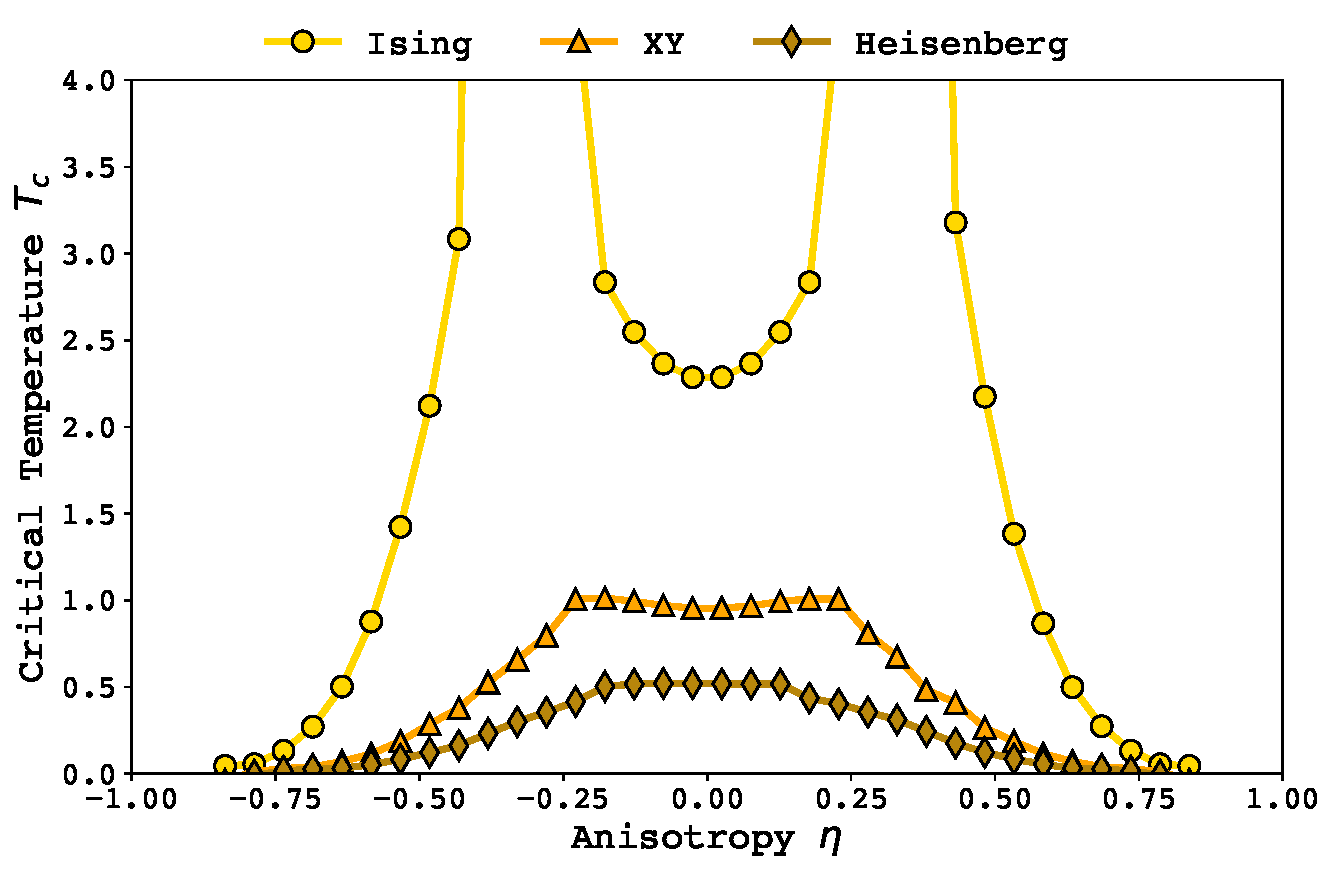
\includegraphics[width=\linewidth]{../figs/rect-phase.pdf}
  \caption{The phase diagram of the rectangular lattice as a function of the anisotropy $\eta$, where $\eta = 0$ is the square lattice and $\eta\rightarrow \pm 1$ is the anisotropic limit.}
  \label{fig:rect}
\end{figure}

A similar procedure shows the phase diagram for the einstein tiling, where $a$ and $b$ are now the two lengths shown in figure \ref{fig:einstein}.

\section{Transverse Ising Model}
\label{sec:tim}

\section{Conclusion}
\label{sec:conclusion}

\appendix

\section{The Fluctuation-Dissipation Theorem and Magnetic Susceptibility}
\label{app:fluctuation-dissipation}


\section{Equivalence Between the Transverse Ising Model and Classical Ising Model}
\label{app:tim-equivalence}

\bibliography{cmt.bib}

\end{document}